\section{Desarrollo}

\subsection{Sintesis mediante polinomios de Chebyshev}

Para sintetizar el filtro, partiremos de los requerimientos 
dados en la planilla, donde podemos observar que se trata de 
un filtro pasa-banda con las siguientes características:

\begin{itemize}
    \item Banda de Paso $B_p$: de $800[Hz]$ a $1250[Hz]$.
    \item Atenuación Máxima en Banda de Paso $A_p$: $0.25[dB]$.
    \item Banda de Rechazo $B_s$: por debajo de $200[Hz]$ y por encima de $5000[Hz]$.
    \item Atenuación Mínima en Banda de Rechazo $A_s$: $30[dB]$.
\end{itemize}

Para el cálculo de la función de transferencia que satisfaga la 
plantilla, se procedió a transformar las frecuencias críticas de 
Hertz a radianes por segundo mediante la relación $\omega = 
2\pi f$:

\begin{itemize}
    \item $\omega_p1 = 2\pi \cdot 800 \approx 5026.55 [rad/s]$.
    \item $\omega_p2 = 2\pi \cdot 1250 \approx 7853.98 [rad/s]$.
    \item $\omega_s1 = 2\pi \cdot 200 \approx 1256.64 [rad/s]$.
    \item $\omega_s2 = 2\pi \cdot 5000 \approx 31415.93 [rad/s]$.
\end{itemize}

Utilizando el script de MATLAB proporcionado por la cátedra, se 
determinó el orden mínimo del filtro para cumplir con una 
atenuación mínima de $30[dB]$ en la banda de rechazo y un 
rizado máximo de $0.25[dB]$ en la banda de paso.\\
El resultado obtenido fue un filtro de orden $4$. Podemos observarlo en la 
siguiente figura y su función de transferencia es:

\begin{figure}[h!]
    \centering
    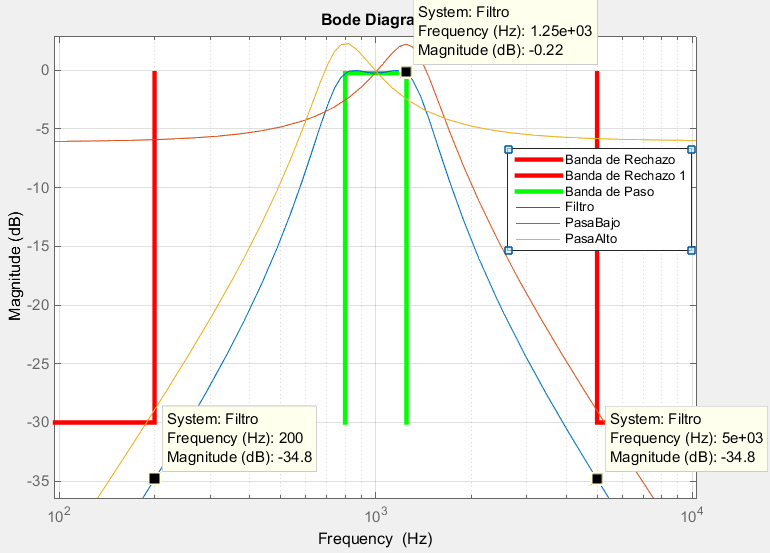
\includegraphics[width=0.8\textwidth]{figures/Desarrollo/Matlab_1.png}
    \caption{Plantilla de diseño del filtro.}
\end{figure}

$$H(s)_{TOTAL} = \frac{1.642 \cdot 10^7 \cdot s^2}{s^4 + 5080 \cdot s^3 + 
9.586 \cdot 10^7 \cdot s^2 + 2.006 \cdot 10^11 \cdot s + 1.559 \cdot 
10^15}$$

Para la implementación física, se descompone esta función de cuarto orden en 
dos etapas bicuadráticas de segundo orden (SOS). Siguiendo la metodología de 
diseño, se identifican una etapa con comportamiento de transferencia 
Pasa-Bajo y otra Pasa-Alto:

$$H(s)_{PB} = \frac{3.284 \cdot 10^7}{s^2 + 3184 \cdot s + 6.632 \cdot 10^7}$$

$$H(s)_{PA} = \frac{0.5 \cdot 10^7}{s^2 + 1896 \cdot s + 2.35 \cdot 10^7}$$



